



\documentclass[a4paper,12pt,spanish]{article}

\usepackage[utf8]{inputenc}


\usepackage{blindtext}
%\usepackage{microtype}
\usepackage{amsfonts, amsmath, amsthm, amssymb}
%\usepackage{fancyhdr}
%\usepackage{index}
%\usepackage{multicol}    

%\usepackage{booktabs}

\usepackage[T1]{fontenc}
\usepackage[utf8]{inputenc}
\usepackage{graphicx}
\usepackage[spanish,es-tabla]{babel}
\usepackage{url}
\usepackage{enumitem}

\usepackage[unicode=true, pdfusetitle,
bookmarks=true,bookmarksnumbered=false,bookmarksopen=false,
breaklinks=true,pdfborder={0 0 1},backref=false,colorlinks=false]
{hyperref}

\usepackage{listings}
\usepackage{longtable}


\usepackage{siunitx} %para el sistema internacional
\usepackage[export]{adjustbox}
\usepackage{booktabs} 
\usepackage{subcaption}

\usepackage{float}


\newcommand{\address}[1]{
	\par {\raggedright #1
		\vspace{1.4em}
		\noindent\par}
}

\usepackage[table,xcdraw]{xcolor}


\pagenumbering{gobble}
\include{noNumberPage}
\pagenumbering{arabic}
\setcounter{page}{8}

%tutorial de tablas latex: https://manualdelatex.com/tutoriales/tablas

\usepackage{multirow}

% \usepackage[table,xcdraw]{xcolor}


%Inicio del documento (hasta que se cierre con \end{document}
\begin{document}
	
	
	\title{Estadística Aplicada a Medidas Nucleares}
	
	%\author{Adrián Rivero Fernández}
	\date{}
	
	\maketitle
	
	
	\section{Objetivos de la práctica}
	
	\vspace{\baselineskip}
	
	1. Determinar la desviación estadística de una serie de medidas de la actividad de una muestra radiactiva.\\
	
	2. Comparar la desviación estadística experimental con la desviación estadística de la distribución de Poisson.\\

	3. Estudiar la fiabilidad estadística del detector Geiger-Müller.\\
	
	
	
	\section{Medidas de la actividad}
	
	Para un tiempo de 10s, tomamos el número de cuentas para distintos voltajes, obteniendo la Tabla 1.
	\begin{table}[H]
		\centering
		\begin{tabular}{|c|c|c|c|c|}
			\cline{1-2} \cline{4-5}
			Medida & Cuentas &  & Medida & Cuentas \\ \cline{1-2} \cline{4-5} 
			1      & 2358    &  & 16     & 2220    \\ \cline{1-2} \cline{4-5} 
			2      & 2247    &  & 17     & 2124    \\ \cline{1-2} \cline{4-5} 
			3      & 2217    &  & 18     & 2272    \\ \cline{1-2} \cline{4-5} 
			4      & 2232    &  & 19     & 2298    \\ \cline{1-2} \cline{4-5} 
			5      & 2209    &  & 20     & 2304    \\ \cline{1-2} \cline{4-5} 
			6      & 2219    &  & 21     & 2149    \\ \cline{1-2} \cline{4-5} 
			7      & 2256    &  & 22     & 2190    \\ \cline{1-2} \cline{4-5} 
			8      & 2247    &  & 23     & 2214    \\ \cline{1-2} \cline{4-5} 
			9      & 2213    &  & 24     & 2189    \\ \cline{1-2} \cline{4-5} 
			10     & 2245    &  & 25     & 2275    \\ \cline{1-2} \cline{4-5} 
			11     & 2257    &  & 26     & 2261    \\ \cline{1-2} \cline{4-5} 
			12     & 2279    &  & 27     & 2208    \\ \cline{1-2} \cline{4-5} 
			13     & 2196    &  & 28     & 2227    \\ \cline{1-2} \cline{4-5} 
			14     & 2258    &  & 29     & 2218    \\ \cline{1-2} \cline{4-5} 
			15     & 2289    &  & 30     & 2251    \\ \cline{1-2} \cline{4-5} 
		\end{tabular}
	\caption{Medidas para 10s}
	\end{table}
	
	\section{Tratamiento de datos}
	
	La cantidad de medidas tomadas es 
	\[N = 30				\]
	
	por lo tanto, los grados de libertad serán
	
	\[f = N - 1 = 29 		\]
	
	La media de impulsos por intervalo es, por tanto, 
	
	\[ \frac{\sum n_i}{N} = 2237,4	\]
	
	Según la distribución de Poisson, la desviación típica de la medida será
	
	\[ s_{teor} = \sqrt{n} = 47,3		\]
	
	La desviación tipica experimental
	
	\[s_{exp} = \sqrt{\frac{\sum (n_i - n)^2}{N - 1}} = 46,67			\]
	
	
	A partir de las desviaciones, obtenemos $\chi^2$	
	\[\chi^2 = \frac{s^2_{exp}}{s^2_{teor}}(N-1) = 28,23			\]
	
	
	Consultando la tabla de la Figura 1, para los 29 grados de libertad que tenemos, y el $\chi^2$ obtenido, vemos que la probabilidad debe ser muy cercana a 0,50
	
	
	
	\[p \simeq 0,50 					\]
	
	
	
	
	
	
\begin{figure}[H]
	\centering
	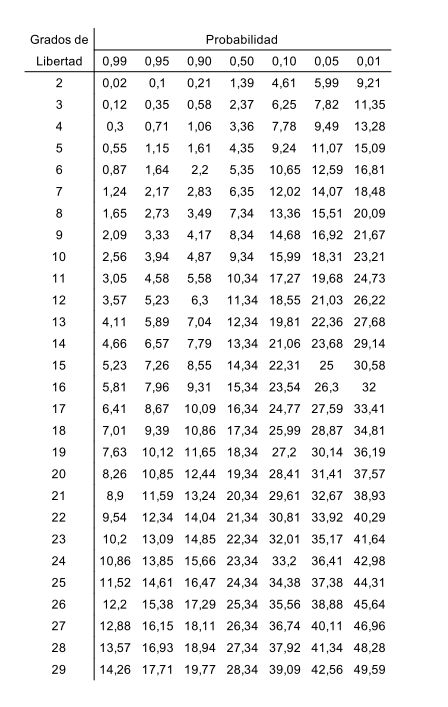
\includegraphics[width=0.6\linewidth]{imagenes/image.FX4PL2}
	\caption{Probabilidad según grados de libertad}
	\label{fig:chicuadrado}
\end{figure}
	
	
	\section{Discusión}
	
	Podemos comprobar como la desviación típica teórica y la experimental son muy similares. De hecho, la diferencia entre ambas respecto a la teórica es de 
	\[ \frac{s_{teor}- s_{exp} }{ s_{teor} } = 0,013 \longrightarrow 1,3\%
	\]
	
	El valor de la probabilidad $p$ a partir del $\chi ^2$ se presenta dentro de los criterios de aceptación
	\[ 0,10 < p \simeq 0,50 < 0,90
	\]

	Por tanto, se puede concluir que existe una correspondencia biunóvica entre el número de sucesos ionizantes $n$ y el número de impulsos detectados $m$, y 
	el detector se considera estadísticamente fiable.
	
	
	
	
%Más cosas por hacer

%	¿Se parecen la desviación típica experimental y la teórica?
%	El valor de la probabilidad p ¿está en concordancia con los criterios de aceptación establecidos?
%	¿Cuál es el estado del detector desde el punto de vista de su fiabilidad estadística?
	
	
	
	
\end{document}